\documentclass[a4paper,14pt]{article}

\usepackage{tikz}
\usetikzlibrary{positioning}

% --- Настройка шрифтов и локализации для XeLaTeX ---
\usepackage{fontspec}
\usepackage{xunicode}
\usepackage{xltxtra}
\usepackage{polyglossia}
\setmainlanguage{russian}
\setotherlanguage{english}
\defaultfontfeatures{Ligatures=TeX}
\setmainfont{Times New Roman}
\newfontfamily\cyrillicfont{Times New Roman}
\setmonofont{Courier New}
\newfontfamily\cyrillicfonttt{Courier New}

% --- Параметры страницы по ГОСТ (левое 3 см, правое 1 см, верхнее и нижнее по 2 см) ---
\usepackage[left=30mm, right=10mm, top=20mm, bottom=20mm]{geometry}

% --- Интервалы и абзацный отступ (1.25 см, 1.5 интервал) ---
\usepackage{indentfirst}
\setlength{\parindent}{1.25cm}
\usepackage{setspace}
\onehalfspacing

% --- Пакеты для таблиц, списков и графики ---
\usepackage{tabularx}
\usepackage{booktabs}
\usepackage{array}
\usepackage{enumitem}
\setlist{nosep, leftmargin=\parindent}
\usepackage{graphicx}

% --- Листинги кода с корректным отображением пробелов в кириллице ---
\usepackage{listings}
\usepackage{xcolor}

\lstset{
    basicstyle=\ttfamily\footnotesize,
    columns=flexible,
    keepspaces=true,
    breaklines=true,
    frame=single,
    tabsize=2,
    showstringspaces=false,
    keywordstyle=\bfseries\color{blue!70!black},
    commentstyle=\itshape\color{green!50!black},
    stringstyle=\color{red!60!black},
    numbers=none
}

% Определение стиля для TypeScript / JavaScript
\lstdefinelanguage{TypeScript}{
  keywords={abstract, any, as, async, await, boolean, break, case, catch, class,
    const, constructor, continue, debugger, declare, default, delete, do,
    else, enum, export, extends, false, finally, for, from, function, get,
    if, implements, import, in, infer, instanceof, interface, is, keyof,
    let, module, namespace, never, new, null, number, object, of, package,
    private, protected, public, readonly, require, return, set, static,
    string, super, switch, symbol, this, throw, true, try, type, typeof,
    undefined, unique, unknown, var, void, while, with, yield},
  morecomment=[l]{//},
  morecomment=[s]{/*}{*/},
  morestring=[b]',
  morestring=[b]",
  morestring=[b]`
}

% --- Оформление заголовков по стандарту ---
\usepackage{titlesec}
\titleformat{\section}[block]
  {\normalfont\bfseries\filright}
  {\hspace{1.25cm}\thesection\quad}
  {0pt}
  {\MakeUppercase}

\titleformat{\subsection}[block]
  {\normalfont\bfseries\filright}
  {\hspace{1.25cm}\thesubsection\quad}
  {0pt}
  {}

\titlespacing*{\section}{0pt}{18pt}{12pt}
\titlespacing*{\subsection}{0pt}{12pt}{6pt}

% Настройка подписей к рисункам и таблицам
\usepackage[tableposition=top,figureposition=bottom]{caption}
\DeclareCaptionLabelSeparator{emdash}{~---~}
\captionsetup[figure]{
  name={Рисунок},
  labelsep=emdash,
  font={small},
  justification=centering,
  singlelinecheck=true
}
\captionsetup[table]{
  name={Таблица},
  labelsep=emdash,
  font={small},
  justification=raggedright,
  singlelinecheck=false
}

% --- Отточие в содержании ---
\usepackage{tocloft}
\renewcommand{\cftsecleader}{\cftdotfill{\cftdotsep}}
\renewcommand{\cfttoctitlefont}{\hfill\bfseries\MakeUppercase}
\renewcommand{\cftaftertoctitle}{\hfill}

\begin{document}

% =========================================================================
% ТИТУЛЬНЫЙ ЛИСТ
% =========================================================================
\begin{titlepage}
    \centering
    {\small МИНИСТЕРСТВО НАУКИ И ВЫСШЕГО ОБРАЗОВАНИЯ РОССИЙСКОЙ ФЕДЕРАЦИИ}\\
    {\scriptsize \textbf{ФЕДЕРАЛЬНОЕ ГОСУДАРСТВЕННОЕ АВТОНОМНОЕ ОБРАЗОВАТЕЛЬНОЕ УЧРЕЖДЕНИЕ ВЫСШЕГО ОБРАЗОВАНИЯ}}\\
    {\bfseries «НАЦИОНАЛЬНЫЙ ИССЛЕДОВАТЕЛЬСКИЙ УНИВЕРСИТЕТ ИТМО»}\\[0.8cm]

    \textbf{Факультет безопасности информационных технологий}\\[0.6cm]

    \textbf{Направление подготовки: 10.03.01 Информационная безопасность} \\
    \textbf{Образовательная программа: «Технологии защиты информации»} \\[0.6cm]

    \textbf{Дисциплина:} \\
    \textit{\textbf{«Информационная безопасность баз данных»}} \\ [1.5cm]

    {\bfseries ОТЧЕТ ПО ЛАБОРАТОРНОЙ РАБОТЕ №4}\\
    \textit{{\bfseries «Реализация уровня приложения с возможностью многопользовательского доступа к созданной БД»}}\\[4cm]

    \begin{flushright}
        \textbf{Выполнил студент(ы):} \\ [0.5em]
        группа.поток ИББД 1.7 \\ [0.5em]
        Пахомов Владимир Юрьевич / \raisebox{-0.3\height}{
\includegraphics[width=1.3cm]{sign1.png}} \\
        {\scriptsize{\textit{ФИО \hspace{2cm} Подпись \hspace{0.3cm}}}} \\ [0.3cm]
        Сивков Иван Александрович / \raisebox{-0.4\height}{
\includegraphics[width=1.1cm]{sign2.jpg}} \\
        {\scriptsize{\textit{ФИО \hspace{2cm} Подпись \hspace{0.3cm}}}} \\ [0.3cm]
        Булин Михаил Михайлович / \raisebox{-0.4\height}{
\includegraphics[width=1.3cm]{sign3.png}} \\
        {\scriptsize{\textit{ФИО \hspace{2cm} Подпись \hspace{0.3cm}}}} \\ [0.3cm]


        \textbf{Проверил:}\\ [0.5em]
        Ярцева Наталия Андреевна / \underline{\hspace{1.5cm}} \\
        {\scriptsize{\textit{ФИО \hspace{2cm} Подпись \hspace{1cm}}}} \\ [1.5cm]

        {\scriptsize \underline{\hspace{4cm}}} \\
        {\scriptsize \textit{Отметка о выполнении (один из вариантов: \\ отлично, хорошо, удовлетворительно, зачтено)}} \\
        {\scriptsize \underline{\hspace{4cm}}} \\
        {\scriptsize \textit{Дата \hspace{1.5cm}}}
    \end{flushright}

    \vfill
    Санкт-Петербург\\
    2026
\end{titlepage}

% =========================================================================
% СОДЕРЖАНИЕ
% =========================================================================
\newpage
\pagestyle{plain}
\setcounter{page}{2}

\begin{center}
    {\bfseries \MakeUppercase{Содержание}}
\end{center}
\vspace{-0.5cm}
\tableofcontents

% =========================================================================
% ВВЕДЕНИЕ
% =========================================================================
\newpage
\begin{center}
    {\bfseries \MakeUppercase{Введение}}
\end{center}
\addcontentsline{toc}{section}{ВВЕДЕНИЕ}

\textbf{Цель работы}: получение практических навыков использования серверных языков программирования, современных объектно-реляционных отображений (ORM), создания защищенного программного интерфейса приложения (API) и веб-интерфейса, обеспечивающего ролевой многопользовательский доступ к реляционной базе данных с соблюдением принципов информационной безопасности.

В рамках лабораторной работы создано полноценное клиент-серверное программное обеспечение для автоматизированной информационной системы морских контейнерных перевозок, база данных которой спроектирована и развернута в лабораторных работах №1--2. Архитектура программного решения включает:
\begin{itemize}
    \item \textbf{Серверную часть (Backend)}: на базе асинхронного веб-фреймворка FastAPI, ORM SQLAlchemy и драйвера Psycopg, реализующую защищенный REST API с токен-ориентированной JWT-аутентификацией;
    \item \textbf{Клиентскую часть (Frontend)}: на базе стека React, TypeScript, Vite и Tailwind CSS, предоставляющую динамический адаптивный веб-интерфейс в соответствии с назначенной пользователю ролью;
    \item \textbf{Слой информационной безопасности и ролевого разграничения}: изоляцию данных грузоотправителей, предоставление специализированных представлений (\textit{VIEW}) и агрегированных аналитических отчетов со сложными соединениями (\textit{JOIN}) и группировками (\textit{GROUP BY}).
\end{itemize}

% =========================================================================
% 1. ВЫБОР СТЕКА ТЕХНОЛОГИЙ И АРХИТЕКТУРА СИСТЕМЫ
% =========================================================================
\newpage
\section{Выбор стека технологий и архитектура системы}

\subsection{Обоснование серверного стека (FastAPI, SQLAlchemy 2.0, Psycopg 3)}
Для реализации прикладного уровня выбрана связка технологий на языке Python:
\begin{itemize}
    \item \textbf{Язык программирования Python 3.14} обеспечивает высокую скорость и безопасность разработки, прозрачность синтаксиса и обширную экосистему библиотек для работы с базами данных и криптографией.
    \item \textbf{Фреймворк FastAPI}: высокопроизводительный асинхронный фреймворк, базирующийся на спецификации ASGI и стандарте OpenAPI/Swagger. Обеспечивает автоматическую строгую валидацию входных/выходных структур данных посредством Pydantic, что предотвращает атаки внедрения некорректных типов данных.
    \item \textbf{ORM SQLAlchemy 2.0}: промышленный стандарт объектно-реляционного маппинга. Использование современной типизированной декларативной модели (\texttt{Mapped}, \texttt{mapped\_column}) полностью исключает риск SQL-инъекций (SQL Injection), так как все формируемые запросы параметризуются на уровне драйвера СУБД.
    \item \textbf{Драйвер Psycopg 3}: современная реализация протокола клиентского взаимодействия с PostgreSQL, поддерживающая расширенные типы данных и высокую скорость выполнения транзакций.
\end{itemize}

\subsection{Обоснование клиентского стека (React 19, TypeScript, Tailwind CSS)}
В качестве платформы пользовательского интерфейса выбран компонентный SPA-подход (Single Page Application):
\begin{itemize}
    \item \textbf{React 19 и TypeScript}: обеспечивают строгую статическую типизацию на клиенте, предотвращая логические ошибки рендеринга и работы с состоянием аутентификации.
    \item \textbf{Vite}: современный инструмент сборки frontend-приложений, обеспечивающий высокую скорость запуска и оптимизацию результирующего бандла.
    \item \textbf{Tailwind CSS v4}: утилитарный CSS-фреймворк для быстрой верстки чистого, адаптивного интерфейса системы с поддержкой темного и светлого режимов отображения.
\end{itemize}

\subsection{Общая архитектура и интеграция с механизмами защиты СУБД}
На рисунке \ref{fig:arch_scheme} представлена трехуровневая архитектура информационной системы.

\begin{figure}[h!]
    \centering
    \begin{tikzpicture}[
            node distance=1.5cm,
            box/.style={rectangle, draw=black, thick, fill=blue!5, text width=4.2cm, align=center, rounded corners, minimum height=1.2cm},
            secbox/.style={rectangle, draw=red!70!black, dashed, thick, fill=red!5, text width=4.2cm, align=center, rounded corners, minimum height=1.2cm},
            arrow/.style={thick, ->, >=stealth}
        ]
        \node (client) [box] {\textbf{React SPA}\\Пользовательский интерфейс (Роли: Client, Dispatcher, Admin)};
        \node (api) [box, below=of client] {\textbf{FastAPI Backend}\\JWT-аутентификация, RBAC, Pydantic-валидация};
        \node (orm) [box, below=of api] {\textbf{SQLAlchemy ORM 2.0}\\Параметризованные запросы, маппинг сущностей};
        \node (db) [secbox, below=of orm] {\textbf{PostgreSQL СУБД}\\Таблицы, VIEW, RLS, Триггеры аудита (main\_log), Шифрование (secret\_data)};

        \draw [arrow] (client) -- node[right]{\footnotesize HTTPS / JSON} (api);
        \draw [arrow] (api) -- node[right]{\footnotesize Python Call} (orm);
        \draw [arrow] (orm) -- node[right]{\footnotesize Psycopg3 (SQL)} (db);
    \end{tikzpicture}
    \caption{Трехуровневая архитектура информационной системы}
    \label{fig:arch_scheme}
\end{figure}

При разработке архитектуры заложен принцип сквозной информационной безопасности:
\begin{enumerate}
    \item На уровне приложения аутентификация осуществляется по стандарту OAuth2 с выдачей JWT-токенов (алгоритм HS256). В токене фиксируется имя субъекта и его системная роль.
    \item Матрица доступа приложения (\texttt{app.access}) строго ограничивает перечень доступных таблиц и допустимых операций (\texttt{read}, \texttt{write}, \texttt{delete}) для каждой роли.
    \item Взаимодействие с базой данных спроектировано с учетом требований ЛР3:
          \begin{itemize}
              \item Любые операции модификации (\texttt{POST}, \texttt{PATCH}, \texttt{DELETE}), инициируемые через API, приводят к выполнению SQL-команд в PostgreSQL, на которые навешаны триггеры логирования, автоматически фиксирующие пользователя, время и дельту данных в служебной таблице аудита.
              \item Конфиденциальные таблицы (таблица секретных ключей и токенов шифрования, исследуемая в рамках симметричного шифрования pgcrypto) исключены из реестра доступных клиентам и диспетчерам отношений, обеспечивая соблюдение принципа наименьших привилегий (PoLP).
          \end{itemize}
\end{enumerate}

% =========================================================================
% 2. ОБЪЕКТНО-РЕЛЯЦИОННОЕ ОТОБРАЖЕНИЕ (ORM SQLALCHEMY)
% =========================================================================
\newpage
\section{Объектно-реляционное отображение (ORM SQLAlchemy)}

В модулях пакета \texttt{app.models} реализовано строго типизированное отображение реляционных таблиц и представлений БД в классы SQLAlchemy 2.0 с использованием типизации \texttt{Mapped} и \texttt{mapped\_column}.

\subsection{Маппинг базовых сущностей предметной области}
Ниже приведен фрагмент декларативного описания сущностей «Заказ» (\textit{Order}) и «Рейс» (\textit{Voyage}) с сохранением целостности связей и проверочных ограничений (\textit{CHECK}), установленных в ЛР2:

\begin{lstlisting}[language=Python]
from datetime import datetime
from decimal import Decimal
from typing import Optional
from sqlalchemy import Integer, String, Numeric, DateTime, ForeignKey, CheckConstraint, func
from sqlalchemy.orm import Mapped, mapped_column, relationship
from app.models.base import Base

class Order(Base):
    __tablename__ = "orders"
    __table_args__ = (
        CheckConstraint("cargo_weight > 0", name="chk_orders_cargo_weight"),
        CheckConstraint("cargo_volume > 0", name="chk_orders_cargo_volume"),
        CheckConstraint("total_price >= 0", name="chk_orders_total_price"),
    )

    id: Mapped[int] = mapped_column(Integer, primary_key=True, autoincrement=True)
    client_id: Mapped[int] = mapped_column(
        Integer, ForeignKey("clients.id", onupdate="CASCADE", ondelete="RESTRICT"), nullable=False
    )
    cargo_name: Mapped[str] = mapped_column(String(150), nullable=False)
    cargo_weight: Mapped[Decimal] = mapped_column(Numeric(10, 2), nullable=False)
    cargo_volume: Mapped[Decimal] = mapped_column(Numeric(10, 2), nullable=False)
    total_price: Mapped[Decimal] = mapped_column(Numeric(12, 2), nullable=False)
    created_at: Mapped[datetime] = mapped_column(DateTime, server_default=func.now(), nullable=False)

    # Отношения к смежным сущностям
    client: Mapped["Client"] = relationship(back_populates="orders")
    invoice: Mapped[Optional["Invoice"]] = relationship(
        back_populates="order", uselist=False, cascade="all, delete-orphan", passive_deletes=True
    )
    order_containers: Mapped[list["OrderContainer"]] = relationship(
        back_populates="order", cascade="all, delete-orphan", passive_deletes=True
    )
    voyage_orders: Mapped[list["VoyageOrder"]] = relationship(
        back_populates="order", cascade="all, delete-orphan", passive_deletes=True
    )
\end{lstlisting}

\subsection{Маппинг представлений (VIEW)}
Для работы с представлениями, созданными в ЛР1 и ЛР2, классы ORM сконфигурированы с метапараметром \texttt{\{"info": \{"is\_view": True\}\}}, что предотвращает попытки создания физических таблиц миграциями и информирует систему о режиме «только чтение»:

\begin{lstlisting}[language=Python]
class ViewClientTracking(Base):
    __tablename__ = "view_client_tracking"
    __table_args__ = {"info": {"is_view": True}}

    order_id: Mapped[int] = mapped_column(Integer, primary_key=True)
    client_id: Mapped[int] = mapped_column(Integer)
    cargo_name: Mapped[str] = mapped_column(String(150))
    vessel_name: Mapped[str] = mapped_column(String(100))
    port_of_loading: Mapped[str] = mapped_column(String(100))
    port_of_discharge: Mapped[str] = mapped_column(String(100))
    departure_date: Mapped[datetime] = mapped_column(DateTime)
    arrival_date: Mapped[datetime] = mapped_column(DateTime)
    voyage_status: Mapped[str] = mapped_column(String(30))

class ViewVoyageManifest(Base):
    __tablename__ = "view_voyage_manifest"
    __table_args__ = {"info": {"is_view": True}}

    voyage_id: Mapped[int] = mapped_column(Integer, primary_key=True)
    ship_name: Mapped[str] = mapped_column(String(100))
    ship_capacity_tons: Mapped[Decimal] = mapped_column(Numeric(10, 2))
    origin_port: Mapped[str] = mapped_column(String(100))
    destination_port: Mapped[str] = mapped_column(String(100))
    total_orders_assigned: Mapped[int] = mapped_column(Integer)
    total_cargo_tons: Mapped[Decimal] = mapped_column(Numeric(10, 2))
\end{lstlisting}

% =========================================================================
% 3. РЕАЛИЗАЦИЯ РОЛЕВОГО МНОГОПОЛЬЗОВАТЕЛЬСКОГО ДОСТУПА
% =========================================================================
\newpage
\section{Реализация ролевого многопользовательского доступа}

\subsection{Матрица разграничения доступа}
В соответствии с концептуальным проектом выделены 3 основные роли пользователей:
\begin{enumerate}
    \item \textbf{Клиент (\textit{client})}~--- грузоотправитель, имеющий доступ исключительно к своим заказам, счетам, трекингу грузов и представлению контейнеров своего заказа. Разрешено создание новых заказов. Доступ к чужим заказам блокируется на уровне фильтрации внешнего ключа \texttt{client\_id}.
    \item \textbf{Диспетчер флота (\textit{dispatcher})}~--- сотрудник логистического центра порта. Имеет доступ к судовому грузовому манифесту, ведомостям безопасности пломб, реестрам судов, портов, контейнеров и рейсов. Обладает полномочиями планирования рейсов (\texttt{write} в \textit{voyages} и \textit{voyage\_orders}).
    \item \textbf{Администратор безопасности (\textit{admin})}~--- обладает полным доступом (\texttt{CRUD}) ко всем сущностям и служебным таблицам базы данных.
\end{enumerate}

Сводная матрица полномочий представлена в таблице \ref{tab:rbac_matrix}.

\begin{table}[h!]
    \caption{Матрица полномочий ролевой модели доступа}
    \label{tab:rbac_matrix}
    \small
    \begin{tabularx}{\textwidth}{|l|X|X|X|}
        \hline
        \textbf{Роль}       & \textbf{Чтение (SELECT / READ)}                                                                                                                                           & \textbf{Создание/Изменение (WRITE)}       & \textbf{Удаление (DELETE)} \\ \hline
        \textbf{client}     & \texttt{view\_client\_orders}, \texttt{view\_client\_tracking}, \texttt{orders}, \texttt{invoices}, \texttt{order\_containers}, \texttt{clients}                          & \texttt{orders}                           & Запрещено                  \\ \hline
        \textbf{dispatcher} & \texttt{view\_voyage\_manifest}, \texttt{view\_container\_safety \_audit}, \texttt{voyages}, \texttt{ships}, \texttt{ports}, \texttt{containers}, \texttt{voyage\_orders} & \texttt{voyages}, \texttt{voyage\_orders} & Запрещено                  \\ \hline
        \textbf{admin}      & Все таблицы и представления                                                                                                                                               & Все физические таблицы                    & Все физические таблицы     \\ \hline
    \end{tabularx}
    \vspace{1mm}
    % \footnotesize $^*$ Чтение записей в таблицах \textit{orders}, \textit{invoices}, \textit{clients} ограничено строками с \texttt{client\_id}, принадлежащим текущему пользователю.
\end{table}

\subsection{Реализация контроля доступа в модуле app.access}
Разграничение прав реализовано централизованно в программном слое backend:

\begin{lstlisting}[language=Python]
ROLE_ACCESS = {
    "client": {
        "read": [
            "view_client_orders", "view_client_tracking", "orders",
            "invoices", "order_containers", "clients"
        ],
        "write": ["orders"],
        "delete": [],
    },
    "dispatcher": {
        "read": [
            "view_voyage_manifest", "view_container_safety_audit", "voyages",
            "ships", "ports", "containers", "voyage_orders"
        ],
        "write": ["voyages", "voyage_orders"],
        "delete": [],
    },
    "admin": {
        "read": list(TABLE_REGISTRY),
        "write": list(DOMAIN_TABLES),
        "delete": list(DOMAIN_TABLES),
    },
}
\end{lstlisting}

При попытке выполнения операции обращения к таблице или строке зависимость \texttt{get\_current\_user} проверяет валидность токена, после чего эндпоинт валидирует право доступа. В случае отсутствия прав клиенту возвращается статус \texttt{HTTP 403 Forbidden}.

% =========================================================================
% 4. СЛОЖНЫЕ АНАЛИТИЧЕСКИЕ ЗАПРОСЫ С GROUP BY
% =========================================================================
% \newpage
\section{Сложные аналитические запросы с группировкой (GROUP BY)}

В соответствии с пунктом 4 задания для каждой выделенной группы пользователей разработан специализированный эндпоинт в модуле \texttt{app.routers.reports}, выполняющий сложный агрегационный запрос к более чем двум сущностям с использованием соединений \texttt{JOIN}, группировки \texttt{GROUP BY} и возможностью сортировки и фильтрации.

\subsection{Аналитический отчет для роли «Клиент»}
Запрос выполняет расчет сводной финансовой статистики и объемов перевозок клиента по статусам оплаты счетов. Задействованы сущности: \textit{clients}, \textit{orders}, \textit{invoices}.

\begin{lstlisting}[language=SQL]
SELECT 
    c.name AS client_name,
    COALESCE(i.payment_status, 'No Invoice') AS invoice_status,
    COUNT(o.id) AS total_orders,
    COALESCE(SUM(o.cargo_weight), 0) AS total_cargo_weight,
    COALESCE(SUM(o.total_price), 0) AS total_declared_price,
    COALESCE(SUM(i.amount), 0) AS total_invoiced_amount
FROM clients c
JOIN orders o ON c.id = o.client_id
LEFT JOIN invoices i ON o.id = i.order_id
WHERE c.id = :client_id
GROUP BY c.name, COALESCE(i.payment_status, 'No Invoice')
ORDER BY total_declared_price DESC;
\end{lstlisting}

\subsection{Аналитический отчет для роли «Диспетчер флота»}
Запрос формирует сводную загрузку портов отправления: число выполненных рейсов, суммарный дедвейт задействованных контейнеровозов и общее количество обработанных заказов. Задействованы сущности: \textit{ports}, \textit{voyages}, \textit{ships}, \textit{voyage\_orders}.

\begin{lstlisting}[language=SQL]
SELECT 
    p.name AS port_name,
    p.country AS country,
    COUNT(DISTINCT v.id) AS total_departures,
    COALESCE(SUM(s.deadweight), 0) AS total_deadweight_serviced,
    COUNT(vo.order_id) AS total_orders_routed
FROM ports p
JOIN voyages v ON p.id = v.departure_port_id
JOIN ships s ON v.ship_id = s.id
LEFT JOIN voyage_orders vo ON v.id = vo.voyage_id
GROUP BY p.name, p.country
HAVING COUNT(DISTINCT v.id) > 0
ORDER BY total_deadweight_serviced DESC;
\end{lstlisting}

\subsection{Аналитический отчет для роли «Администратор»}
Глобальный мониторинг использования флота по типам и флагам приписки судов с подсчетом перевезенных объемов и выручки. Задействованы сущности: \textit{ships}, \textit{voyages}, \textit{voyage\_orders}, \textit{orders}.

\begin{lstlisting}[language=SQL]
SELECT 
    s.flag_state,
    s.name AS ship_name,
    COUNT(DISTINCT v.id) AS total_voyages,
    COUNT(vo.order_id) AS total_orders_loaded,
    COALESCE(SUM(o.cargo_weight), 0) AS total_weight_carried,
    COALESCE(SUM(o.total_price), 0) AS gross_revenue
FROM ships s
LEFT JOIN voyages v ON s.id = v.ship_id
LEFT JOIN voyage_orders vo ON v.id = vo.voyage_id
LEFT JOIN orders o ON vo.order_id = o.id
GROUP BY s.flag_state, s.name
ORDER BY gross_revenue DESC;
\end{lstlisting}

% =========================================================================
% 5. ДЕМОНСТРАЦИЯ РАБОТЫ И ИНТЕРФЕЙС ПОЛЬЗОВАТЕЛЯ
% =========================================================================
\newpage
\section{Демонстрация работы пользовательского интерфейса}

\subsection{Аутентификация и вход под разными ролями}
Для подтверждения многопользовательского режима в базу данных добавлены преднастроенные учетные записи:
\begin{itemize}
    \item \texttt{balttrade} (пароль: \texttt{client123}, роль: \textit{client}, привязан к \textit{client\_id = 1});
    \item \texttt{dispatcher} (пароль: \texttt{dispatcher123}, роль: \textit{dispatcher});
    \item \texttt{admin} (пароль: \texttt{admin123}, роль: \textit{admin}).
\end{itemize}

Форма авторизации (\texttt{/login}) передает учетные данные в формате \\ \texttt{application/x-www-form-urlencoded} на эндпоинт \texttt{/api/v1/login}, получая подписанный JWT токен.

\begin{figure}[h!]
    \centering
    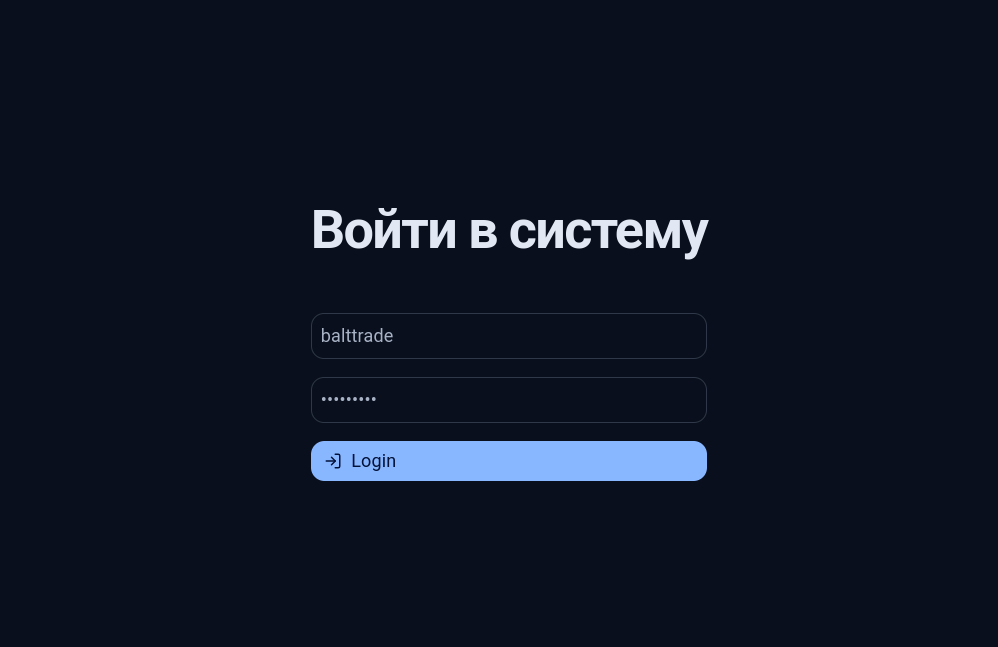
\includegraphics[width=0.9\textwidth]{web1.png}
    \caption{Окно аутентификации в пользовательском интерфейсе}
    \label{fig:ui_login}
\end{figure}

\subsection{Ограничение списка таблиц в зависимости от учетной записи}
После успешной аутентификации клиент запрашивает профиль пользователя через \texttt{/api/v1/me} и динамический список доступных таблиц через \texttt{/api/v1/tables}:
\begin{itemize}
    \item Пользователю \texttt{balttrade} доступны только 6 объектов: представления \texttt{view\_client\_orders}, \\ \texttt{view\_client\_tracking} и таблицы \texttt{orders}, \texttt{invoices}, \texttt{order\_containers}, \texttt{clients}. Кнопка добавления записи активна только для таблицы \texttt{orders}.
    \item Диспетчеру доступны технологические представления манифеста и таблицы рейсов, судов, портов и контейнеров.
    \item Администратор видит полный реестр объектов с включенной возможностью редактирования и удаления.
\end{itemize}

\begin{figure}[h!]
    \centering
    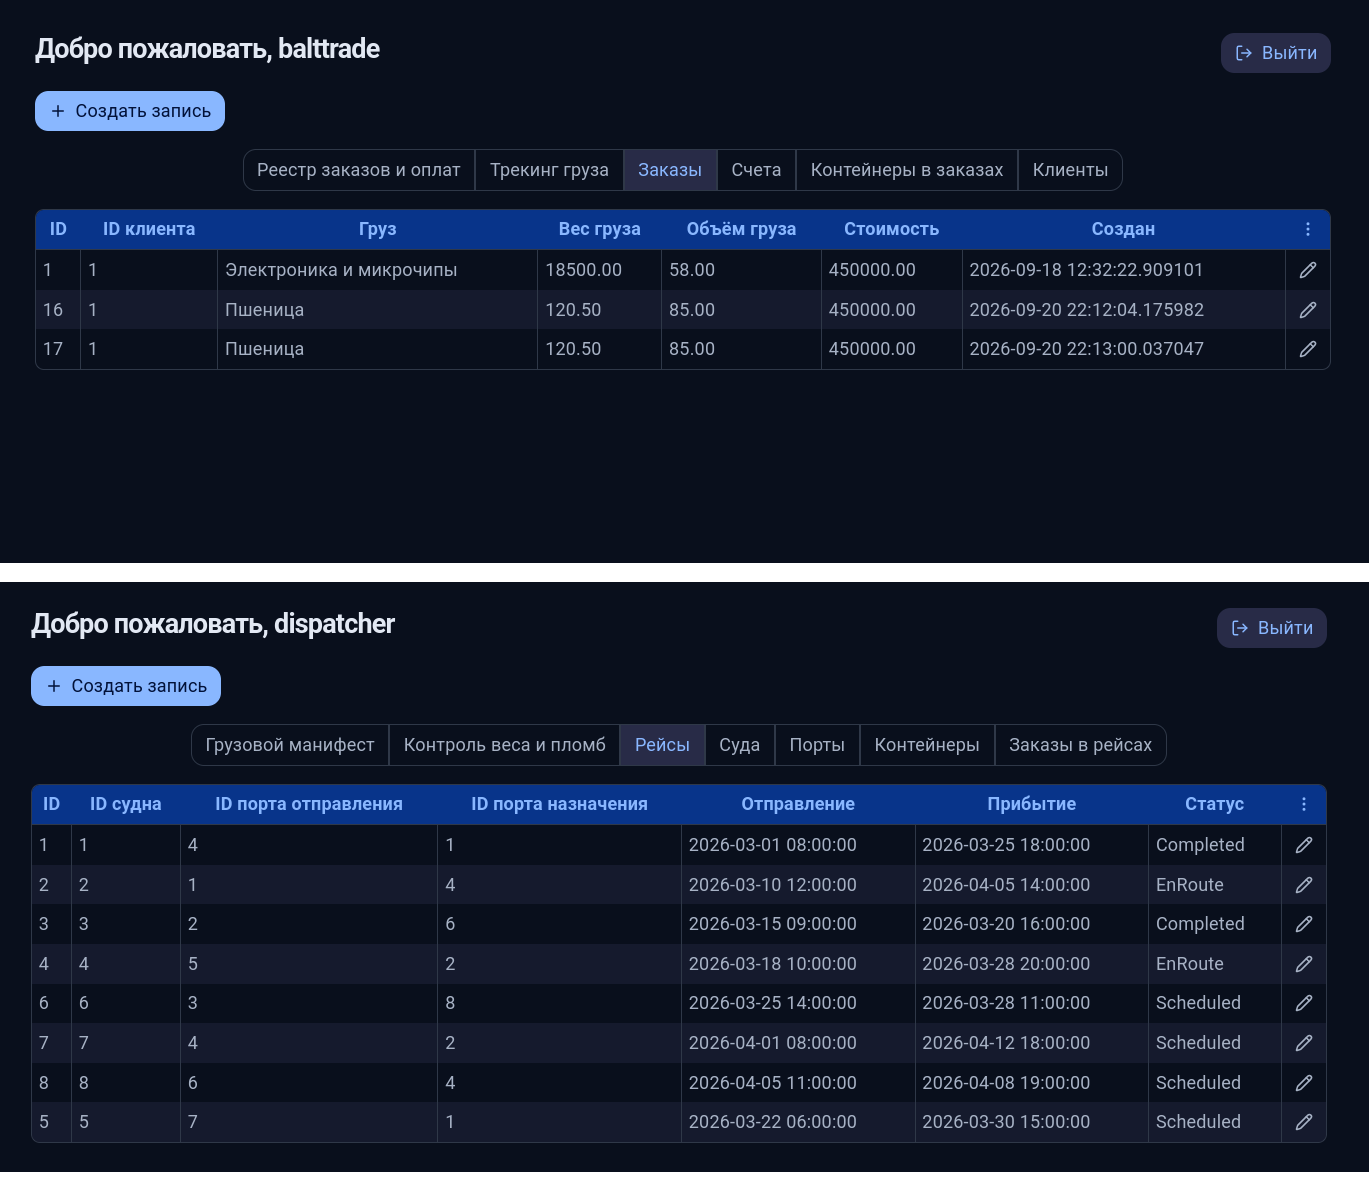
\includegraphics[width=0.9\textwidth]{web2.png}
    \caption{Отображение доступных таблиц в пользовательском интерфейсе в зависимости от роли пользователя}
    \label{fig:ui_tables}
\end{figure}

\newpage

\subsection{Выполнение операций CRUD и отражение в триггерах аудита}
При создании нового заказа клиентом (рисунок \ref{fig:ui_create}) отправляется запрос \texttt{POST /api/v1/tables/orders}. Вспомогательный обработчик backend автоматически подставляет авторизованный \texttt{client\_id}, исключая возможность фальсификации отправителя.

\begin{figure}[h!]
    \centering
    % \fbox{\begin{minipage}{0.9\textwidth}
    %         \centering
    %         \vspace{3mm}
    %         \textbf{Интерфейс создания записи (Роль: Client)}\\[2mm]
    %         \begin{tabular}{|l|l|}
    %             \hline
    %             \textbf{Поле}         & \textbf{Значение}               \\ \hline
    %             Наименование груза    & Комплектующие серверных станций \\ \hline
    %             Вес груза (кг)        & 14200.00                        \\ \hline
    %             Объем груза (м$^3$)   & 42.50                           \\ \hline
    %             Общая стоимость (руб) & 390000.00                       \\ \hline
    %         \end{tabular}
    %         \vspace{3mm}
    %     \end{minipage}}
    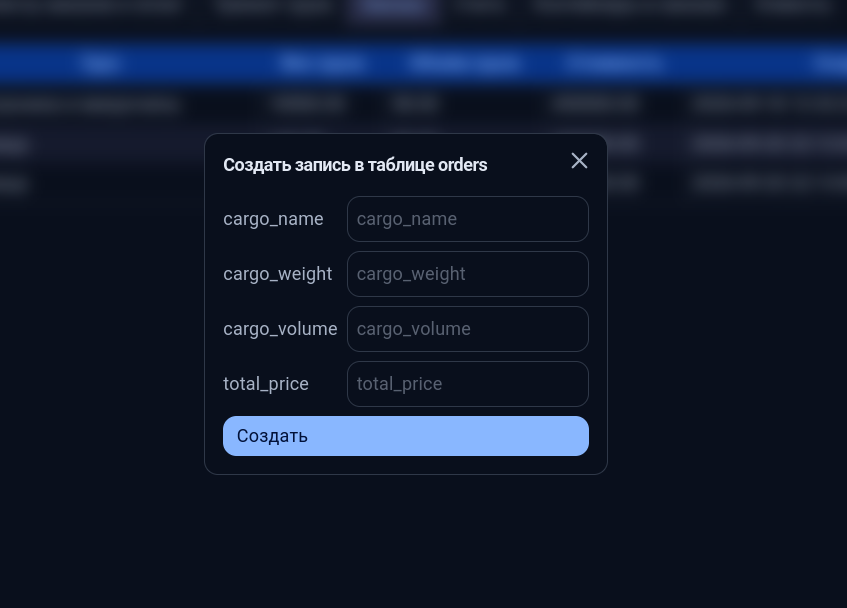
\includegraphics[width=0.9\textwidth]{web3.png}
    \caption{Модальное окно создания заказа в пользовательском интерфейсе}
    \label{fig:ui_create}
\end{figure}

На уровне PostgreSQL в результате данной транзакции срабатывает триггер мониторинга БД, вносящий в таблицу логов \texttt{main\_log} запись с типом \texttt{'I'}, меткой \texttt{now()}, текущим пользователем и JSON-представлением созданного кортежа.

При попытке несанкционированного доступа (например, запросе диспетчером финансовых счетов клиентов через \texttt{GET /api/v1/tables/invoices}) сервер возвращает:
\begin{lstlisting}[language=SQL]
HTTP/1.1 403 Forbidden
{"detail": "Недостаточно прав для чтения таблицы invoices"}
\end{lstlisting}

% =========================================================================
% 6. ЛИСТИНГИ КЛЮЧЕВЫХ МОДУЛЕЙ СИСТЕМЫ
% =========================================================================
\newpage
\section{Листинги ключевых модулей системы}

\subsection{Контроллер таблиц и CRUD операций (backend/app/routers/tables.py)}
\begin{lstlisting}[language=Python]
from typing import Any
from fastapi import APIRouter, Depends, HTTPException, Query, status
from sqlalchemy import desc, select
from sqlalchemy.orm import Session

from app.access import can_delete, can_read, can_write, is_view, readable_tables
from app.db import get_db
from app.deps import get_current_user
from app.models import AppUser, Order
from app.schemas import RowPayload, TableListResponse
from app.tables import get_model, serialize_row

router = APIRouter(tags=["tables"])

@router.get("/tables")
def list_available_tables(user: AppUser = Depends(get_current_user)) -> dict[str, list[dict]]:
    tables = []
    for name in readable_tables(user.role):
        tables.append({
            "name": name,
            "kind": "view" if is_view(name) else "table",
            "can_write": can_write(user.role, name),
            "can_delete": can_delete(user.role, name),
        })
    return {"tables": tables}

@router.get("/tables/{table_name}", response_model=TableListResponse)
def read_table_data(
    table_name: str,
    limit: int = Query(default=100, ge=1, le=1000),
    user: AppUser = Depends(get_current_user),
    db: Session = Depends(get_db),
) -> TableListResponse:
    if not can_read(user.role, table_name):
        raise HTTPException(status_code=status.HTTP_403_FORBIDDEN, detail="Доступ запрещен")
    
    model = get_model(table_name)
    stmt = select(model)
    # Фильтрация контекста клиента
    if user.role == "client":
        if hasattr(model, "client_id") and user.client_id:
            stmt = stmt.where(model.client_id == user.client_id)
        elif table_name == "clients" and user.client_id:
            stmt = stmt.where(model.id == user.client_id)
            
    rows = db.scalars(stmt.limit(limit)).all()
    return TableListResponse(table=table_name, items=[serialize_row(r) for r in rows], count=len(rows))

@router.post("/tables/{table_name}", status_code=status.HTTP_201_CREATED)
def create_row(
    table_name: str,
    payload: RowPayload,
    user: AppUser = Depends(get_current_user),
    db: Session = Depends(get_db),
) -> dict:
    if not can_write(user.role, table_name) or is_view(table_name):
        raise HTTPException(status_code=status.HTTP_403_FORBIDDEN, detail="Запись запрещена")
    
    model = get_model(table_name)
    data = payload.model_dump()
    if user.role == "client" and table_name == "orders":
        data["client_id"] = user.client_id
        
    instance = model(**data)
    db.add(instance)
    db.commit()
    db.refresh(instance)
    return serialize_row(instance)
\end{lstlisting}

\subsection{Модуль отчетов со сложными запросами (backend/app/routers/reports.py)}
\begin{lstlisting}[language=Python]
from fastapi import APIRouter, Depends, HTTPException, status
from sqlalchemy import desc, func, select
from sqlalchemy.orm import Session
from app.db import get_db
from app.deps import get_current_user
from app.models import AppUser, Client, Invoice, Order, Port, Ship, Voyage, VoyageOrder
from app.schemas import ReportResponse

router = APIRouter(prefix="/reports", tags=["reports"])

@router.get("/client", response_model=ReportResponse)
def get_client_report(user: AppUser = Depends(get_current_user), db: Session = Depends(get_db)):
    if user.role != "client" or not user.client_id:
        raise HTTPException(status_code=status.HTTP_403_FORBIDDEN, detail="Доступно только клиенту")

    stmt = (
        select(
            Client.name.label("client_name"),
            func.coalesce(Invoice.payment_status, "Не выставлен").label("payment_status"),
            func.count(Order.id).label("total_orders"),
            func.coalesce(func.sum(Order.cargo_weight), 0).label("total_weight"),
            func.coalesce(func.sum(Order.total_price), 0).label("total_price"),
        )
        .join(Order, Client.id == Order.client_id)
        .outerjoin(Invoice, Order.id == Invoice.order_id)
        .where(Client.id == user.client_id)
        .group_by(Client.name, func.coalesce(Invoice.payment_status, "Не выставлен"))
        .order_by(desc("total_price"))
    )
    res = db.execute(stmt).mappings().all()
    return ReportResponse(
        role="client",
        title="Сводная статистика заказов клиента",
        description="Группировка заказов по статусам оплаты",
        items=[dict(r) for r in res],
        count=len(res)
    )
\end{lstlisting}

\subsection{Главный интерфейсный модуль React (frontend/src/pages/main.tsx)}
\begin{lstlisting}[language=TypeScript]
import { useEffect, useState, useCallback } from "react";
import { Navigate, useNavigate } from "react-router";
import { LogOut, Plus } from "lucide-react";
import { RowDialog } from "../components/row-dialog";
import { TableLayout } from "../components/table-layout";
import { TablesBar } from "../components/tables-bar";
import type { TableInfo, Table, User } from "../types/types";
import { fetchTables, fetchTable, createRow, deleteRow, updateRow } from "../utils/tables";

export function Main() {
  const navigate = useNavigate();
  const [token, setToken] = useState(localStorage.getItem("token"));
  const [rowDialogOpen, setRowDialogOpen] = useState(false);
  const [user, setUser] = useState<User | null>(null);
  const [tablesInfo, setTablesInfo] = useState<TableInfo[]>([]);
  const [selectedTable, setSelectedTable] = useState<Table | null>(null);

  const getTable = useCallback(async (tableName: string) => {
    if (!token) return;
    const data = await fetchTable(token, tableName);
    const info = tablesInfo.find((t) => t.name === tableName);
    setSelectedTable({
      name: tableName,
      kind: info?.kind ?? "table",
      can_write: info?.can_write ?? false,
      can_delete: info?.can_delete ?? false,
      count: data.count,
      items: data.items,
    });
  }, [token, tablesInfo]);

  useEffect(() => {
    if (!token) return;
    async function load() {
      const meRes = await fetch("/api/v1/me", { headers: { Authorization: `Bearer ${token}` } });
      if (!meRes.ok) { localStorage.removeItem("token"); setToken(null); return; }
      setUser(await meRes.json());
      setTablesInfo(await fetchTables(token!));
    }
    void load();
  }, [token]);

  if (!token) return <Navigate to="/login" replace />;

  return (
    <main className="max-w-6xl mx-auto pt-16">
      <div className="flex justify-between items-center">
        <h2>Добро пожаловать, {user?.username} ({user?.role})</h2>
        <button className="bg-secondary-container px-3 py-1.5 rounded-md" onClick={() => {
          localStorage.removeItem("token"); navigate("/login");
        }}><LogOut className="w-4 h-4" /> Выйти</button>
      </div>
      <TablesBar tablesInfo={tablesInfo} selectedTable={selectedTable} getTable={getTable} />
      {selectedTable && (
        <TableLayout
          tableName={selectedTable.name}
          columns={Object.keys(selectedTable.items[0] ?? {})}
          items={selectedTable.items}
          canWrite={selectedTable.can_write}
          canDelete={selectedTable.can_delete}
        />
      )}
    </main>
  );
}
\end{lstlisting}

% =========================================================================
% ЗАКЛЮЧЕНИЕ
% =========================================================================
\newpage
\begin{center}
    {\bfseries \MakeUppercase{Заключение}}
\end{center}
\addcontentsline{toc}{section}{ЗАКЛЮЧЕНИЕ}

В ходе выполнения лабораторной работы был успешно разработан и развернут уровень клиент-серверного приложения с организацией ролевого многопользовательского доступа к базе данных «Информационная система морских контейнерных перевозок».

Основные результаты работы:
\begin{enumerate}
    \item Обоснован выбор архитектурного стека (Python/FastAPI, SQLAlchemy 2.0, PostgreSQL, React 19, Vite, Tailwind CSS), обеспечивающего высокую надежность, производительность и защищенность данных от атак типа SQL-инъекций и несанкционированного доступа.
    \item Выполнен полный маппинг 9 реляционных отношений и 4 представлений в структуру классов ORM с сохранением ограничений целостности.
    \item Спроектирована и реализована ролевая система доступа (RBAC) для трех категорий субъектов (\textit{client}, \textit{dispatcher}, \textit{admin}). Доступ к чтению, модификации и удалению данных строго разграничен.
    \item Реализованы сложные аналитические SQL-запросы с соединением более чем трех сущностей и группировкой (\textit{GROUP BY}), позволяющие вычислять коммерческие показатели рейсов и сводную статистику грузопотока.
    \item Создан веб-интерфейс, динамически адаптирующий доступные таблицы, формы добавления данных и панели аналитических отчетов под полномочия вошедшего пользователя.
    \item Архитектура приложения полностью согласована с механизмами защиты СУБД (триггерный аудит и криптографическая защита): операции модификации вызывают срабатывание триггеров аудита в PostgreSQL, а секретные таблицы изолированы от неавторизованных ролей.
\end{enumerate}

\end{document}